\subsection*{Risici}
Vi har valgt at analysere vores project i forhold bohms model, samt at lave risici analyse p� forskellige muligheder mht. teknologi heriblandt: Android og Windows mobile, eventuelt kunne vi ogs� have overvejet mobile web. For hver enkelt teknologi skal overvejes specielt i forhold vores erfaring med den, samt relevans ift. m�let. \\


\begin{figure}[H]
\begin{center}
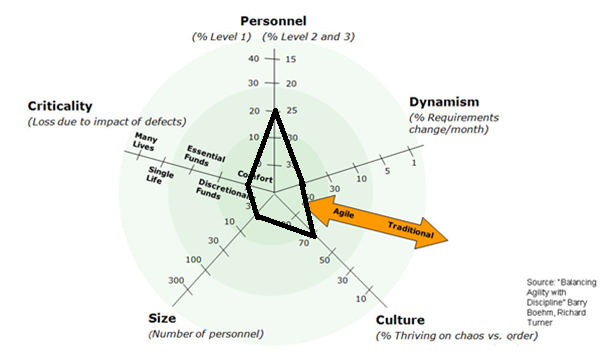
\includegraphics[scale=1.00]{includes/billeder/bohmsmodel.png}
\caption{Bohms model}
\label{fig:risici:bohms_model}
\end{center}
\end{figure}

\subsection*{Bohms model ~\ref{fig:risici:bohms_model}} 
Vi en lille gruppe p� 3, med kun 2 udviklere. Det er ikke kritisk om hvorvidt appen skulle crashe s� vi har vurderet Criticality til Comfort. For Personnel har vi vurderet til at ligger cirka midt p� idet at vi har meget forskelligt fagligt niveau i forhold til kodning. Vi forventer at der bliver brug for meget dynamik, idet at vi har lidt kendskab til teknologierne og at der derfor h�jst sandsynligt vil opst� en masse �ndringer undervejs i processen. I gruppen trives vi med en lille smule overordnet planl�gning, men ellers p� kaos og h�j personlig frihed.

\subsection*{Risici analyse}
Vi har valgt at fokusere p� risici for Android og Windows mobile idet at vi mener at disse er blandt de mest relevante teknologier i forhold til vores app. Yderligere kunne man evt. vurdere for IPhone og mobile web.

\subsubsection*{Android mobile}
\begin{figure}[H]
\begin{center}
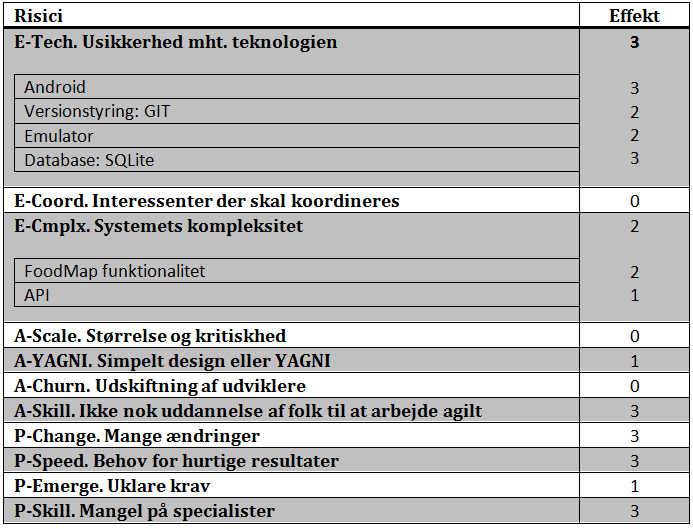
\includegraphics[scale=0.70]{includes/billeder/risici_analyse_android.png}
\caption{Risici analyse android}
\label{fig:risici:analyse_android}
\end{center}
\end{figure}

\textsf{Omgivelser (Enviroment):} ~\ref{fig:risici:analyse_android} \\
Vi har vurderet at der er h�j usikkerhed mht. teknologien specielt ift. Android og SQLite. Der er ikke nogen interessenter der skal koordineres. Systemets kompleksitet vil have en moderat effekt, mest er det FoodMap funktionaliteten som kan vise sig problematisk da vi ikke helt ved hvad den indeb�rer, samt at der vil forekomme nogle performance og usability krav der hurtigt kan g�re systemet komplekst. \\ 
\textsf{E-risici ialt:} 3 + 0 + 2 = 5
\\ \\


\textsf{Agile A-risici:} ~\ref{fig:risici:analyse_android} \\
Umiddelbart er det er et relativt sm�t projekt, derfor har vi vurderet A-Scale til ikke at have nogen effekt. Simpelt design vil ikke have den store effekt, da der ikke beh�ves den store planl�gning eller dokumentation af systemet. Der vil ikke v�re nogen udskiftning af udviklere s� A-Churn har ingen effekt. A-Skill kan g� hen at f� en stor effekt, idet at vores uddannelsesniveau er meget lavt i forhold til teknologien. \\ \\    
\textsf{A-risici ialt:} 0 + 1 + 0 + 3 = 4 \\ \\

\textsf{Plan-driven P-risks:} ~\ref{fig:risici:analyse_android} \\
Vi forventer at der vil forekomme mange �ndringer og dette vil have en stor effekt. Derudover er der et behov for hurtige resultater, idet at vi har brug for l�bende releases for at f� feedback fra reviews. Uklare krav vil have en meget lille effekt, idet at det i h�j grad er os selv der definerer dem. Mangel p� specialister vil have en stor effekt, da specialiser er n�dvendige for at kunne bruge de plandrevne v�rkt�jer ordentligt med den p�g�ldende teknologi. \\
\textsf{P-risici ialt:} 3 + 3 + 1 + 3 = 10

\newpage

\subsubsection*{Windows mobile} 
\begin{figure}[H]
\begin{center}
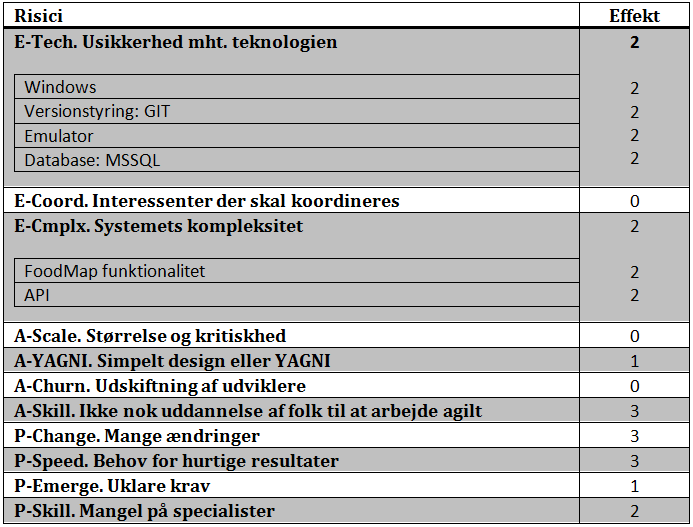
\includegraphics[scale=0.70]{includes/billeder/risici_analyse_windowsphone.png}
\caption{Risici analyse windowsphone}
\label{fig:risici:analyse_windowsphone}
\end{center}
\end{figure}

\textsf{Omgivelser (Enviroment):} ~\ref{fig:risici:analyse_windowsphone} \\
Vi har vurderet at der er j�vn usikkerhed mht. teknologien idet at vi ikke den store viden for Windows mobile, dog har vi tidligere erfaring med Visual studio og MSSQL. Der er ikke nogen interessenter der skal koordineres. Systemets kompleksitet vil have en moderat effekt, mest er det FoodMap funktionaliteten som kan vise sig problematisk da vi ikke helt ved hvad den indeb�rer, samt at der vil forekomme nogle performance og usability krav der hurtigt kan g�re systemet komplekst. \\ \\
\textsf{Enviroment effekt ialt:} \\
2 + 0 + 2 = 4 \\ \\

\textsf{Agile A-risici} og \textsf{Plan-driven P-risks:} ~\ref{fig:risici:analyse_windowsphone} \\
Umiddelbart er vilk�rene de samme som for Android mobile, men idet at vi har arbejdet mere med .NET, Visual studio og MSSQL forinden har vi valgt at vurdere effekten p� P-Skill lavere. \\
\textsf{A-risici ialt:} \\
0 + 1 + 0 + 3 = 4 \\

\textsf{P-risks ialt:} \\
3 + 3 + 1 + 2 = 9

\section*{Metodevalg}
Da vi er en lille gruppe som har det bedst med at der ikke er en for stram process og meget personlig frihed under ansvar, foretr�kker vi en meget agil udviklingsmetode og process. \\
Man m� ud fra vores risici-analyse konkludere at vi har meget usikkerhed med teknologien og at det derfor vil v�re en god ide at s�rge for at f� noget kvalitetssikring ind over udviklingen, gerne i form af unit testing.
Det ser umiddelbart ud som om at Windows mobile er nemmere at tilg�, men idet at Android markedet har flere brugere, finder vi det mere relevant at arbejde med.

\newpage

\subsection*{Projektplanl�gning og styring}
Iterationsplan og releaseplan, burndown chart

\subsection*{Kvalitetssikring og test}
Vi benytter pair programming og dokumentation. \\
Vi har valgt ikke at benytte Unit testing, alfa/betatests og continuous integration fordi ...

\subsection*{Deployment og konfigurationsstyring}
Omkring at ops�tte og teste softwaren kundens systemer. Kan g�res med forskelligt mellemrum afh�ngigt af metode.

\newpage

\subsection*{Velocity}

Vi forventer at have 4 timer om dagen per mand i gruppen. Dvs. 8 mandetimer om dagen med 2 hold. \\
4 dage f�rste uge. \\
4 dage anden uge. \\
5 dage tredje uge. \\

5 storypoint (standard) tager 8 mandetimer \\
5/8 = 0,625 storypoint per mandetime \\

%dette skal �ndres...
40 mande timer i en iteration
40*0,625 = 25 storypoints per uge
			5 storypoints per dag \\

4 sprints i alt.

\newpage

\subsection*{Sprint 0}
Sprint 0 benyttede vi til at lave produktbacklog, iterationsplan og burndown. Samt at lave spike p� interfacet til foodmappet. \\
Vi skulle ogs� have lavet spike p� database men n�ede det ikke. \\ 
I �vrigt var Bjarke var ikke tilstede hverken onsdag, torsdag og fredag pga. Gr�n IT.

\subsection*{Sprint 1 med XP}
Til sprint 1 havde vi lavet et burndown som viste storypoints per mandedage. \\
Vi benyttede pair-programming og fokuserede p� de 2 user-stories: \\
\begin{itemize}
\item Kunden vil gerne have flere forslag til ingredienser frem p� food map, ved at trykke p� den midterste knap.
\item Kunden vil gerne have adgang til database.
\end{itemize}

Hvor der indgik database design, oprettelse af tabeller og gui samt generel funktionalitet til foodmap ... \\
Vi l�b ind i et problem med at vores userstory for databasen var for bredt defineret, hvilket resulterede i at vi ikke kunne tegne vores burndown ned. Vi valgte derfor i starten af sprint 2 at dele den op. Derudover delte vi ogs� andre store userstories op...

\newpage

Backloggen s� i sprint 1 s�dan ud:
%link til at genere tabeller: http://www.tablesgenerator.com/
\begin{table}[h]
\begin{tabular}{llll}
Userstory                                                                                                                                                                    & \begin{tabular}[c]{@{}c@{}}Story-\\ points\end{tabular} & \begin{tabular}[c]{@{}c@{}}Mande-\\ timer\end{tabular} & Prioritet                \\ \hline
\multicolumn{1}{|l}{\begin{tabular}[c]{@{}c@{}}Kunden vil gerne have flere forslag til\\ ingredienser frem p� food map, ved at\\ trykke p� den midterste knap.\end{tabular}} & \multicolumn{1}{|l}{3}                                  & \multicolumn{1}{|l}{3}                                 & \multicolumn{1}{|l|}{1}  \\ \hline
\multicolumn{1}{|l}{\begin{tabular}[c]{@{}c@{}}Kunden vil have et animeret foodmap, \\ hvor ingredienser popper ud fra den\\ eksisterende ingrediensbobbel.\end{tabular}}    & \multicolumn{1}{|l}{}                                   & \multicolumn{1}{|l}{}                                  & \multicolumn{1}{|l|}{2}  \\ \hline
\multicolumn{1}{|l}{\begin{tabular}[c]{@{}c@{}}Kunden vil gerne kunne fjerne og tilf�je\\ ingredienser i food map.\end{tabular}}                                             & \multicolumn{1}{|l}{}                                   & \multicolumn{1}{|l}{}                                  & \multicolumn{1}{|l|}{3}  \\ \hline
\multicolumn{1}{|l}{\begin{tabular}[c]{@{}c@{}}Kunden vil gerne have en liste over forskellige\\ opskrifter som er udvalgt af \\ de anf�rte ingredienser.\end{tabular}}      & \multicolumn{1}{|l}{}                                   & \multicolumn{1}{|l}{}                                  & \multicolumn{1}{|l|}{4}  \\ \hline
\multicolumn{1}{|l}{\begin{tabular}[c]{@{}c@{}}Kunden vil gerne have hurtig s�geforslag \\ til ingredienser. (Performance)\end{tabular}}                                     & \multicolumn{1}{|l}{}                                   & \multicolumn{1}{|l}{}                                  & \multicolumn{1}{|l|}{5}  \\ \hline
\multicolumn{1}{|l}{\begin{tabular}[c]{@{}c@{}}Kunden vil gerne have listet opskrifter med\\ billeder, beskrivelse, ingredienser og \\ tilberedning.\end{tabular}}           & \multicolumn{1}{|l}{}                                   & \multicolumn{1}{|l}{}                                  & \multicolumn{1}{|l|}{6}  \\ \hline
\multicolumn{1}{|l}{\begin{tabular}[c]{@{}c@{}}Kunden vil gerne kunne f� et hurtigt overblik\\  over indk�bs- og pr�perationsliste ved opskrift.\end{tabular}}               & \multicolumn{1}{|l}{}                                   & \multicolumn{1}{|l}{}                                  & \multicolumn{1}{|l|}{7}  \\ \hline
\multicolumn{1}{|l}{\begin{tabular}[c]{@{}c@{}}Kunden vil gerne have en menu til navigering\\ i appen.\end{tabular}}                                                         & \multicolumn{1}{|l}{}                                   & \multicolumn{1}{|l}{}                                  & \multicolumn{1}{|l|}{8}  \\ \hline
\multicolumn{1}{|l}{\begin{tabular}[c]{@{}c@{}}Kunden vil gerne kunne gemme indk�bsliste\\ i indk�bsoversigt.\end{tabular}}                                                  & \multicolumn{1}{|l}{}                                   & \multicolumn{1}{|l}{}                                  & \multicolumn{1}{|l|}{9}  \\ \hline
\multicolumn{1}{|l}{\begin{tabular}[c]{@{}c@{}}Kunden vil gerne kunne gemme opskrifter i\\ favoritter.\end{tabular}}                                                         & \multicolumn{1}{|l}{}                                   & \multicolumn{1}{|l}{}                                  & \multicolumn{1}{|l|}{10} \\ \hline
\multicolumn{1}{|l}{\begin{tabular}[c]{@{}c@{}}Kunden vil gerne have en s�rskilt indk�bsliste,\\  som kan tilg�s fra hovedmenuen.\end{tabular}}                              & \multicolumn{1}{|l}{}                                   & \multicolumn{1}{|l}{}                                  & \multicolumn{1}{|l|}{11} \\ \hline
\end{tabular}
\end{table}


\subsection*{Sprint 2}
Vi lavede en ny burndown som viste mandetimer per mandedage. \\
Vi splittede vores userstories og produktbacklog bedre op, samt lavede nye estimater i b�de storypoint og mandetimer p� hver enkelt userstory. Derudover satte vi ogs� tidsestimater p� vores tasks for bedre at v�re i stand til at afslutte tasks og at kunne tegne vores burndown ned. \\
Sprintet kom i h�j grad til at handle om userstories for at lave database samt kobling af database og foodmap.

\subsection*{Product backlog}
Backlog lavet den 9.12.2013 i starten af sprint 2. \\
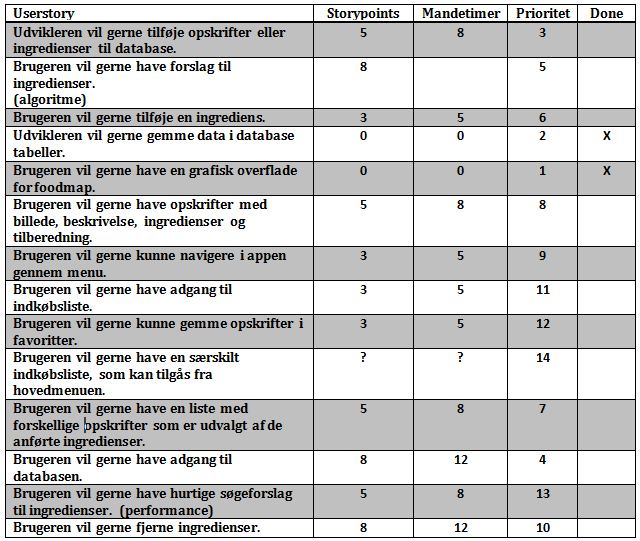
\includegraphics[scale=0.60]{includes/billeder/productbacklog_sprint2.png}

\subsection*{Sprint 3}